Toward synthesizing a multispectral dataset, we showcase the UI2I transformation between a panchromatic modality, \ie, a wide-band thermal image, and a single monochromatic modality, \ie, a narrow-band thermal image.
More concretely, we transform images with a bandwidth of $7 - 14 \mu m$ to images with a central wavelength of $9\mu m$ and a full width at half maximum (FWHM) of $0.5 \mu m$.
For ease of notation, we will use the subscripts \emph{pan} to describe panchromatic data, and \emph{mono} for monochromatic.
This concept could be easily extended to synthesize a complete multispectral dataset by applying it repeatedly for disjoint sub-bands of the thermal spectrum to full coverage.
\subsection{Physical estimator}

\subsubsection{Background}
Black-body radiation is the thermal electro-magnetic signal that is emitted by an ideal opaque object due to its temperature.
Planck's law of black-body radiation states that:
\begin{equation} \label{eq:Plancks-law}
  B_{\lambda}(T) = \frac{2\pi hc^2}{\lambda^5}\frac{1}{e^{\frac{hc}{\lambda kT}} - 1} \; \; \left[W sr^{-1} m^{-2} \mu m^{-1}\right]
\end{equation}
where $B_{\lambda}(T)$ is the ideal object's spectral radiance density, $h$ is Planck's constant, $c$ is the speed of light in a vacuum, $k$ is the Boltzmann constant, $\lambda$ is the electromagnetic wavelength and $T$ is the object's absolute temperature \cite{FundamentalsOfInfraredThermalImaging}.
The Stefan-Boltzmann law \cite{surhone2010stefan} ties the power radiated from an object (which is the result of integrating $B_{\lambda}(T)$ over the entire spectrum of wavelengths from zero to infinity) to the object's temperature:
\begin{equation} \label{eq:stephan-boltzmann-ideal}
    P(T) = \int_0^\infty B_{\lambda}(T) d\lambda = \frac{\sigma}{\pi} T^4 \; \;\left[W sr^{-1} m^{-2}\right]
\end{equation}
where $P$ is the radiated power and $\sigma$ is the Stephan-Boltzmann constant. 

A real-world opaque object emits less power than an ideal black body at the same temperature. 
The ratio between the radiation emission of an object and that of an ideal blackbody at the same temperature is called \emph{emissivity}.
The emissivity is a function of various a-priori unpredictable characteristics of the object, such as material type, surface structure, viewing angle, \etc.
Thus, the Stephan-Boltzmann law for practical objects is given by:
\begin{equation} \label{stephan-boltzmann-practical}
  P(T) =  \frac{\sigma}{\pi} \epsilon T^4 \; \; \left[W sr^{-1} m^{-2}\right]
\end{equation} 
where $\epsilon$ is the object's emissivity.
In general, the emissivity is a function of the wavelength \cite{kerekes2008spectral}, but it is used here as a constant that reflects its expected value over the thermal bandwidth for simplification.

According to \cite{FundamentalsOfInfraredThermalImaging}, when acquired by a thermal microbolometric camera with a finite bandwidth, the incident power on the microbolometer (the thermal camera's sensor) can be described by:
\begin{equation} \label{BolometerIncidentPower}
  \phi(T) = \gamma F_\mathit{pan} \epsilon T^4 \; \; \left[W sr^{-1} m^{-2}\right]
\end{equation}
where $\phi$ is the incident power on the microbolometer, $\gamma$ is a constant governed by the camera's geometrical properties and $F_\mathit{pan}$ represents the fraction of power that is within the camera's bandwidth.
When applying an IR bandpass filter over the camera lens, equation \ref{BolometerIncidentPower} still holds except that $F_\mathit{pan}$ is replaced by $F_\mathit{mono}$, reflecting the fraction of power that is strictly within the bandpass region of the applied filter \cite{FundamentalsOfInfraredThermalImaging}.

Since $\gamma, F_\mathit{pan}, \epsilon$ are all constants, they can be reduced into a single coefficient:
\begin{equation} \label{BolometerIncidentPowerSimplified}
  \phi(T) = a T^4 \; \; \left[W sr^{-1} m^{-2}\right]
\end{equation}
suggesting that the incident power is proportional to $T^4$.
Consequently, a thermally stabilized camera operating in radiometric mode, \ie, when the image intensity levels are linear in the incident power, the intensity of a pixel is obtained by an affine transformation of $T^4$:
\begin{equation} \label{eq:naiveAffineTrans}
  I(T) = b + a T^4
\end{equation}
where $I$ is the intensity level of the pixel and $b$ is the digital bias level. 

Based solely on equation \ref{eq:naiveAffineTrans}, we can seemingly infer an object's temperature directly from the thermal image intensity and vice versa.
However, when dealing with an uncooled (non-thermally stabilized) microbolometric camera, the coefficients in the equation are highly sensitive to the camera's intrinsic temperature. 
According to \cite{10.1117/1.OE.52.6.061304}, the dependency of those coefficients on the intrinsic temperature can be faithfully approximated by a third-order polynomial, concluding that a more accurate description of a pixel's intensity level is
\begin{equation} \label{IntensityVsTemperatures}
  I(T_\mathit{obj}, T_\mathit{int}) = p^{(0)}_c(T_\mathit{int}) + p^{(1)}_c(T_\mathit{int}) T^4_\mathit{obj}
\end{equation}
where $T_\mathit{obj}$ is the object's absolute temperature, $T_\mathit{int}$ is the camera's intrinsic temperature at the time of acquisition, and:
\begin{equation} \label{poly_formula}
  p^{(i)}_c(T_\mathit{int}) = \sum_{k=0}^3  c_{i,k} T_\mathit{int}^k
\end{equation}
where the superscript $^{(i)}$ indicates that the two polynomials in equation \ref{IntensityVsTemperatures} have different coefficients.
Plugging equation \ref{poly_formula} into \ref{IntensityVsTemperatures} and simplifying all of the terms gives:
\begin{equation} \label{eq:full_expr}
  \begin{split}
    I(T_\mathit{obj}, T_\mathit{int}) &= c_{0,0} + c_{0,1} \cdot T_\mathit{int} + c_{0,2} \cdot T^2_\mathit{int} \\
    & + c_{0,3} \cdot T^3_\mathit{int} + (c_{1,0} + c_{1,1} \cdot T_\mathit{int} \\
    & + c_{1,2} \cdot T^2_\mathit{int} + c_{1,3} \cdot T^3_\mathit{int}) \cdot T^4_\mathit{obj} \\
    &= <F, C>
  \end{split}
\end{equation}
where in the last transition, we factorize the relationship as an inner product by stacking all monomials in a single feature vector $F$ and all coefficients in a vector $C$.
Overall, the estimator in equation \ref{eq:full_expr} is made up of eight different monomials and parametrized by eight corresponding coefficients.

\subsubsection{Estimator modeling}
Traditionally, the coefficients from equation \ref{IntensityVsTemperatures} are calibrated to estimate an object's temperature given a measured intensity.
However, we noticed that it could also be used in the opposite direction, \ie, to produce a thermal image intensity given a known object temperature. 
Our innovation is in combining the two directions of applying equation \ref{IntensityVsTemperatures} in a cascade to assemble an analytic UI2I translation model in the following way: 

Given a set of calibrated panchromatic coefficients, we can estimate the object's temperature using the panchromatic intensity and the intrinsic temperature at acquisition:
\begin{equation} \label{eq:backward_poly}
  \hat{T}_\mathit{obj} = \sqrt[4]{\frac{I_\mathit{pan} - p^{(0)}_{c_\mathit{pan}}(T_\mathit{pan})}{p^{(1)}_{c_\mathit{pan}}(T_\mathit{pan})}}
\end{equation}
With the estimated object temperature at hand, we can invoke equation \ref{IntensityVsTemperatures} once again, this time using calibrated monochromatic coefficients, to estimate the monochromatic intensity:
\begin{equation} \label{eq:forward_poly}
  \hat{I}_\mathit{mono} = p^{(0)}_{c_\mathit{mono}}(T_\mathit{mono}) + p^{(1)}_{c_\mathit{mono}}(T_\mathit{mono}) \hat{T}_\mathit{obj}^4
\end{equation}
We treat the cascaded utilization of equations \ref{eq:backward_poly} and \ref{eq:forward_poly} as the physical estimator, and denote it by $G_{\mathit{phys}}$. Formally:
\begin{equation}
  \hat{I}_\mathit{mono} = G_{\mathit{phys}}(I_\mathit{pan}, T_\mathit{pan}, T_\mathit{mono})
\end{equation}

\subsubsection{Estimator coefficient calibration} \label{subsubsec:calibration}
Our in-house-designed calibration setup consists of a thermal camera, blackbody target (to control the scene's temperature) and an environmental chamber (to control the camera's ambient temperature).
The setup was used to capture images of varying scenes and ambient temperatures, to cover the three-dimensional $T_\mathit{int}$-$T_\mathit{obj}$-intensity space.
We then used the measurements to solve for the physical estimator's coefficients using a least-squares minimization criterion.
The calibration results of an exemplary pixel can be visualized as a surface in the three-dimensional $T_\mathit{int}$-$T_\mathit{obj}$-intensity space, as shown in Figure \ref{physical_model_fit}.
\begin{figure}
  \centering
  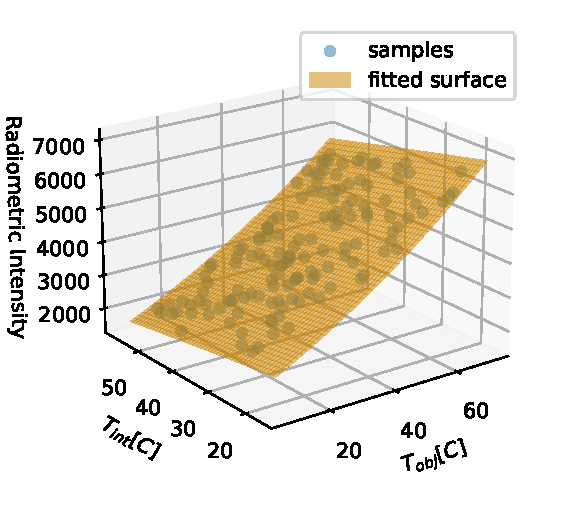
\includegraphics[width=\linewidth]{../figs/methods/physical_model_tight.pdf}
  \caption{An example surface fit visualizing the calibrated polynomial coefficients of a single pixel.}
  \label{physical_model_fit}
\end{figure}
Since the physical estimator requires both panchromatic and monochromatic calibrated coefficients, the calibration process was conducted twice, with and without applying an IR bandpass filter over the camera lens.
For a more elaborate description of the calibration process, please refer to section \ref{Supp-sec:calibration} in the supplementary material.

As it turns out, the calibrated physical estimator was not very accurate, and in particular suffered from a significant first-order error.
Those inaccuracies might have had to do with issues related to the calibration setup, which would normally require an exhaustive investigation to find its root cause.
To circumvent this cumbersome effort, we applied a pixel-wise affine transformation to the estimator, \ie: 
\begin{equation}
  \tilde{G}_{\mathit{phys}} = A \circ G_{\mathit{phys}} + B
\end{equation}
where $A, B$ are matrices and $\circ$ is the Hadamard product operator.
By constructing the elements of the matrices $A, B$ as learnable parameters, back-propagation can be utilized to implicitly correct the physical estimator's prediction of the monochromatic output.


\subsection{Deep estimator}
Given the calibrated physical estimator, one might wonder why this is not enough to solve the UI2I task altogether. 
Unfortunately, as evident from equation \ref{stephan-boltzmann-practical}, the emissivity can utterly change the incident thermal radiation on the camera's sensor. 
Therefore, two objects sharing the exact same temperature might result in significantly different bolometric readouts, and thus different intensity levels \cite{holman1989heat}.
In addition, the application of an IR filter over the lens results in a scene-dependent spatial distortion known as the narcissus effect \cite{FundamentalsOfInfraredThermalImaging}.
This effect is easily observable in real monochromatic images, such as those in Figure \ref{fig:phys_est_gap} in the monochromatic image.
Hence, the physical estimator alone cannot accurately predict the intensity levels of a real-world scene, because it has no capacity to handle scene conditions that are different from its calibration setup.
A demonstration of the gap between the estimated output of the physical estimator and a real monochromatic image appears in figure \ref{fig:phys_est_gap}.

\begin{figure}
  \begin{subfigure}[b]{0.15\textwidth}
      \centering
      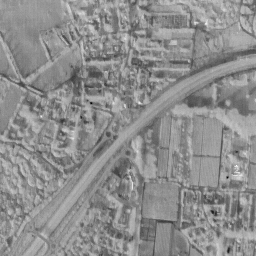
\includegraphics[width=\textwidth]{../figs/outputs/pan/591.png}
      \subcaption{Panchromatic}
      \label{fig:pan_in}
  \end{subfigure}
  \hfill
  \begin{subfigure}[b]{0.15\textwidth}
      \centering
      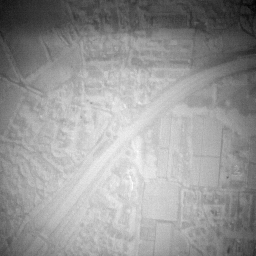
\includegraphics[width=\textwidth]{../figs/outputs/physical/591.png}
      \subcaption{Physical}
      \label{fig:phys_in}
  \end{subfigure}
  \hfill
  \begin{subfigure}[b]{0.15\textwidth}
      \centering
      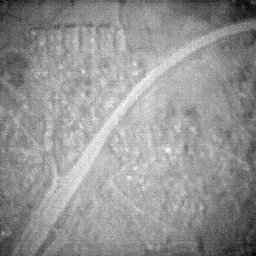
\includegraphics[width=\textwidth]{../figs/outputs/mono/508.png}
      \subcaption{Monochromatic}
      \label{fig:real_our}
  \end{subfigure}
  \hfill

  \caption{Demonstration of the Narcissus effect and the difference between the physical estimator's output and real monochromatic images. (a) Panchromatic (Pan) input. (b) Physical estimator (Phys) output. (c) Real unpaired monochromatic image for reference.}
  \label{fig:phys_est_gap}

\end{figure}

This is where the family of deep generative I2I translation models, which have significantly greater capacity than the polynomial physical estimator, is brought into play.
As baselines, we examined the architectures of CycleGAN \cite{CycleGAN2017} and CUT \cite{park2020cut}, which are considered to achieve SOTA results for the task of UI2I translation.
Both CycleGAN's and CUT's generators consist of a convolutional encoder-decoder scheme with a bottleneck of residual blocks \cite{He2016DeepRL} in between, as schematized in Figure \ref{fig:backbone_models}.

As previously stated in equation \ref{IntensityVsTemperatures}, the intensity levels of both our input and target modalities are affected by the camera's intrinsic temperature.
Fortunately, each image acquired by the FLIR Tau2 is saved along with the intrinsic thermal sensor readouts.
Specifically for our activity, we chose to use the focal plane array temperature as our intrinsic temperature ($T_\mathit{int}$).
Hence, it made sense to design an architecture that could accept this temperature as additional input.
More concretely, we provide the panchromatic (input) intrinsic temperature to the encoder, and the monochromatic (output) intrinsic temperature to the decoder\footnote{In CycleGAN, the generator translating back from the monochromatic to the panchromatic domain receives the inputs in the reverse order, \ie, monochromatic temperature to the encoder and panchromatic temperature to the decoder}.
In doing so, we attempt to disentangle the intrinsic-temperature-dependent transformations (handled by the encoder and decoder) and the more general inter-modal transformation (handled by the bottleneck).

Our use of the intrinsic temperatures as inputs can be thought of as an extension of the concept of conditional GAN (CGAN) \cite{mirza2014conditional}.
In our case, the output is conditioned on two continuous variables (panchromatic and monochromatic intrinsic temperatures) as opposed to the original paper where a single discrete conditional variable was used.
Since both the encoder and decoder are convolutional networks, the intrinsic temperatures (scalars) were reshaped as constant matrices before being concatenated to the corresponding tensors.

\subsection{Fusion of estimators}
Although somewhat mitigated by the learnable affine transformation, the calibrated physical estimator still suffers from inaccuracies.
Nevertheless, its prediction is much closer to the expected monochromatic output than a sheer random guess, which is the initial state of all ordinary GAN generators.
Hence, we can use the physical estimator to produce a prior approximation of the desired output, and let the deep estimator learn the residual \wrt the desired result.
This approach is expected to facilitate the deep estimator's pursuit of the optimal solution and make it more robust \wrt random weight initialization.
Therefore, our proposed method fuses the physical estimator (augmented with the affine transformation) with the deep estimator:
\begin{equation} \label{eq:genFuse}
  G_{\mathit{PETIT}}(x) = \tilde{G}_\mathit{phys}(x) + G_\mathit{deep}(x)
\end{equation}
where $G_\mathit{deep}$ is used to describe the generator of the deep estimator.
Schematics comparing the generator architecture of the deep baseline models (CycleGAN, CUT) and our model (PETIT) are shown in Figure \ref{fig:arch_comp}.

\def \schematicScale {0.79}
\begin{figure*}
  \centering
  \begin{subfigure}{\schematicScale\textwidth}
    \centering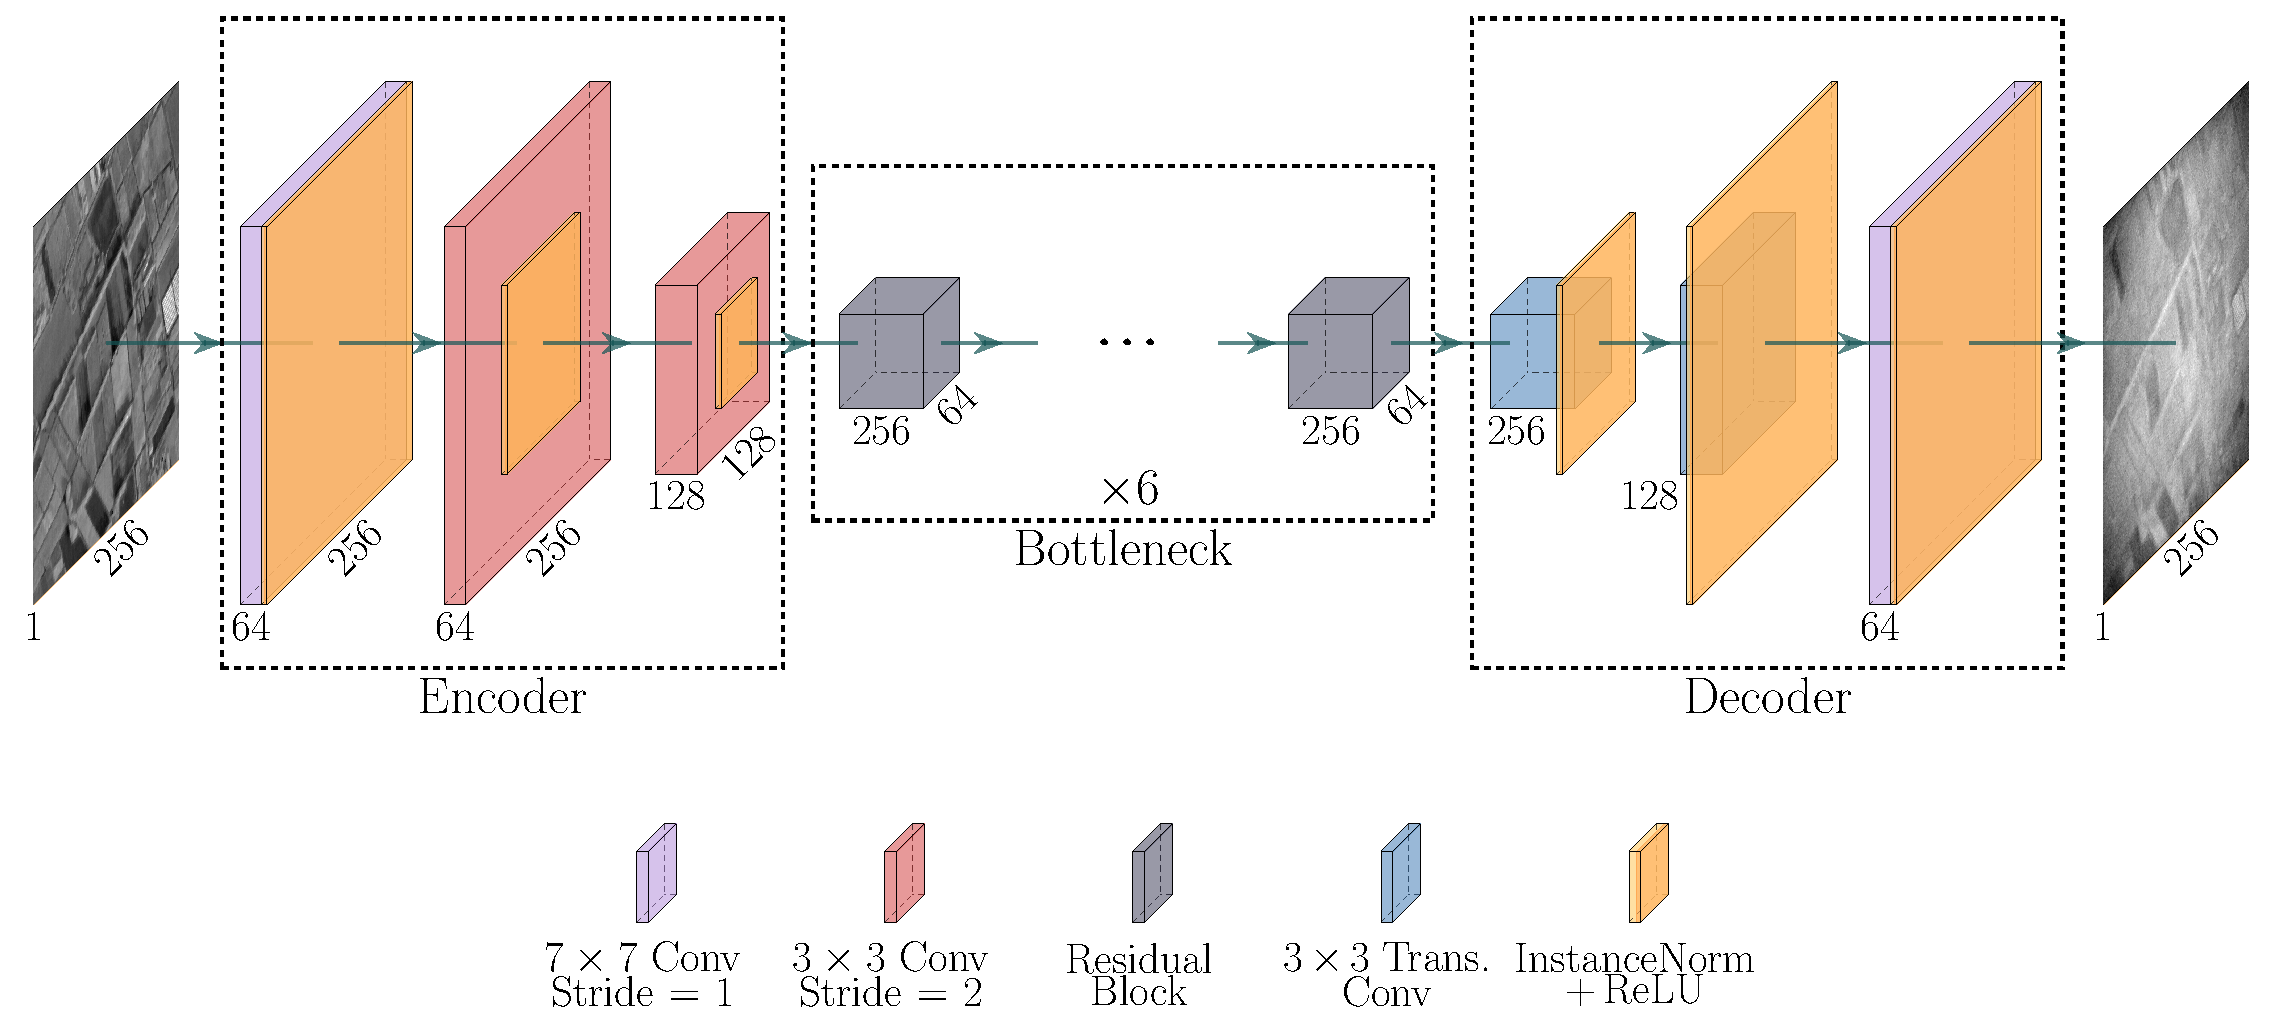
\includegraphics[width=\linewidth]{../figs/network/src/cut.pdf}
    \subcaption{Baseline}
    \label{fig:backbone_models}
    \vspace{0.0cm}
  \end{subfigure}  
  \begin{subfigure}{\schematicScale\textwidth}
    \centering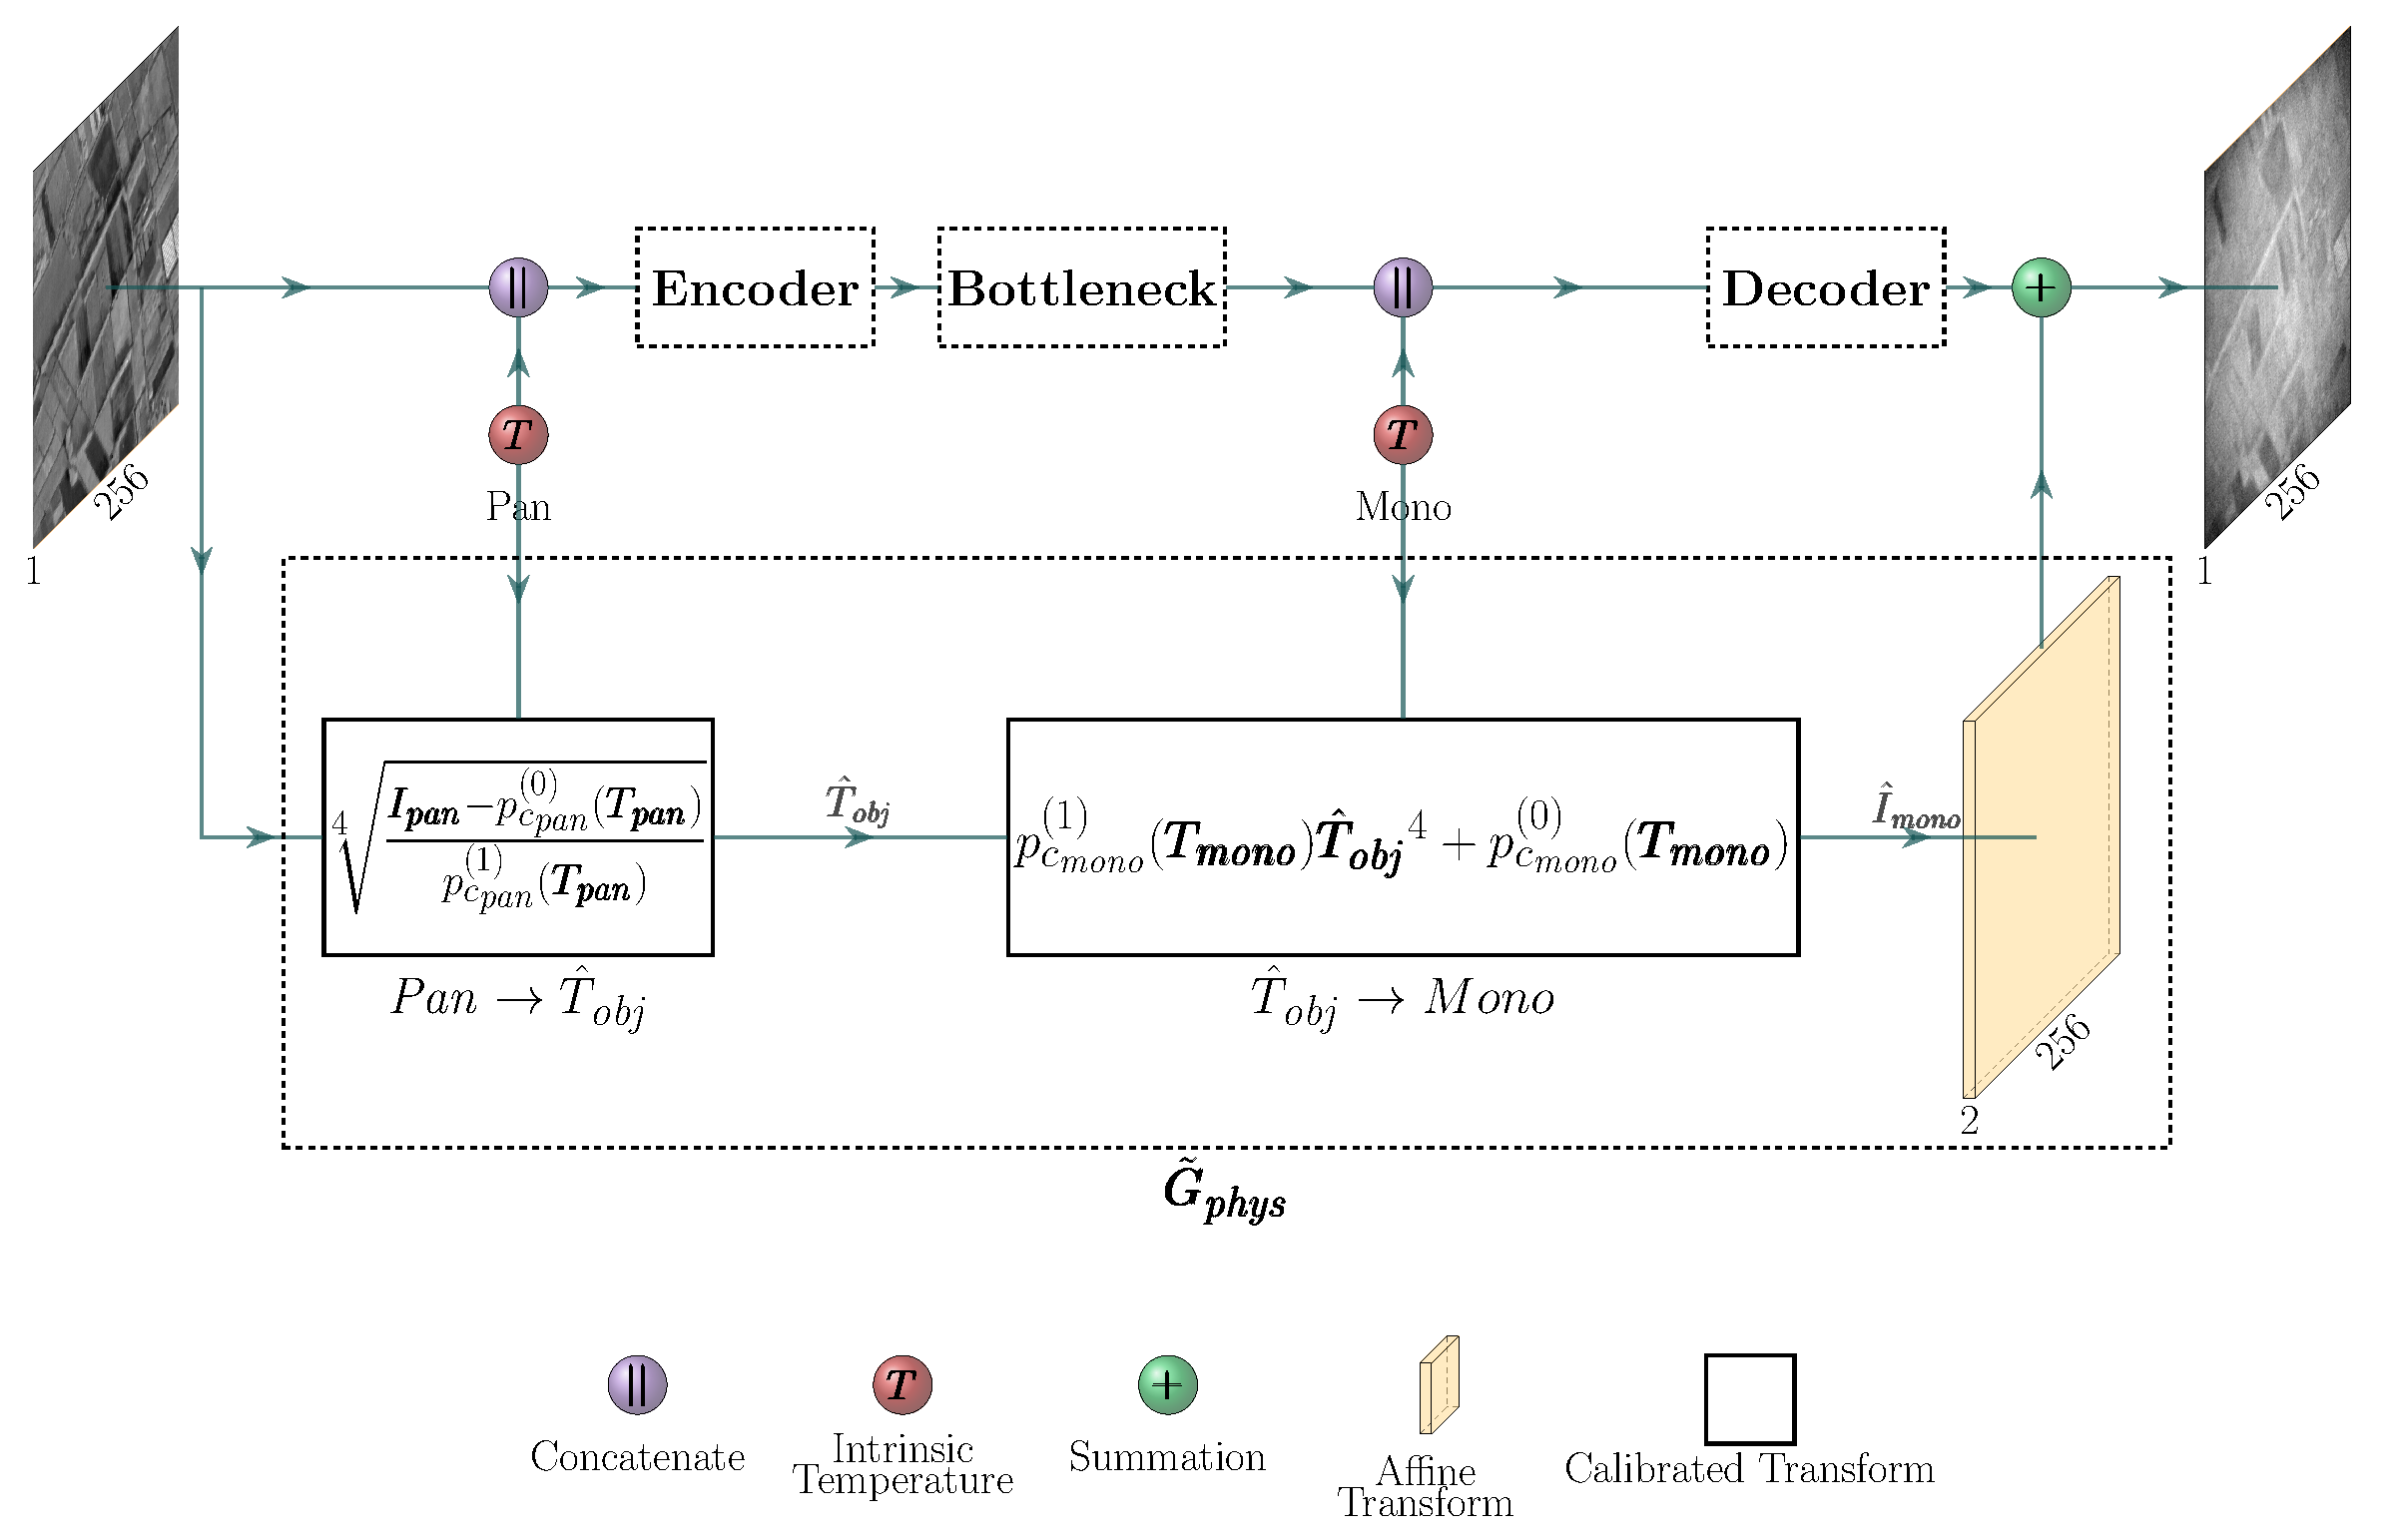
\includegraphics[width=\linewidth]{../figs/network/src/petit.pdf}
    \subcaption{PETIT}
    \label{fig:PETIT_model}
  \end{subfigure}
  \caption{Comparison between the baseline (CycleGAN, CUT) and PETIT (our method) generators. The architectures of the encoder, bottleneck and decoder blocks are identical in all models.}
  \label{fig:arch_comp}
\end{figure*}